% Lines that start with a % are comments and are not included when the LaTeX file is converted to a pdf

% Set up the document class - this can be changed if a different format is required 
\documentclass[12pt,a4paper]{article}
\usepackage[utf8]{inputenc}
\usepackage{amsmath}
\usepackage{amsfonts}
\usepackage{amssymb}
\usepackage{graphicx}
\usepackage[left=2cm,right=2cm,top=2cm,bottom=2cm]{geometry}


% Include packages that contain additional features, for example including special mathematical characters and images in your document
\usepackage{enumerate}
\usepackage{pdfpages}
% The beginning of the document...
\begin{document}

% Please change the following accordingly...
\centerline{\LARGE \textbf{Exercises sheet 6}}\vspace{0.5em}
\centerline{\large by Maximilian Richter and Christian Heppe}\vspace{2em}

% Split the different exercises into different sections...
\section*{Exercise 2}

% To include a plot it must be in the same directory as the .tex file.
\begin{enumerate}[i)]
	\item For the given formula of the time derivative of a population\\
	\begin{equation} 
	\frac{dN}{dt}=rN(1-N/K)-\frac{BN^2}{A^2+N^2}  
	\end{equation}\\ 
	to begin analyzing the postive Parameters $r, K, A$ and $B$ we started by requiring the dimension of $N$ being the number of inhabitants ($"[N]\equiv\#"$) of the population. Thus we find that:\\
	\begin{equation}
		[\frac{dN}{dt}]=\#t^{-1}=[r]\#(1-\frac{\#}{[K]})-[B]\frac{\#^2}{[A]^2+\#^2}
	\end{equation}\\ 
	We assume that $K$ gives us the maximum capacity of the habitat $\implies [K]=\#$ 
	\begin{equation}
		\Leftrightarrow \#t^{-1}=[r]\#-[B]\frac{\#^2}{[A]^2+\#^2}
		\implies [r]=t^{-1} \land [A]=\#
	\end{equation}\\ 
	Which gives us a second (predatory/harmful) population $A$ inside the habitat.
	\begin{center}
		$\implies [B]=\#t^{-1}$
	\end{center}
	With $B$ being the rate of the external reduction of the observed poplation $N$ through $A$ scaled by the factor $\frac{N^2}{A^2+N^2}$\\ 
	To convert the formula into a non-dimensional form we'll use $n=\frac{N}{A}$ as non-dimensional form of $N$. Since we are required to define the non-dimensional $t$ without $r$ we have to use $B$. We decide to define $\tau$ as non-dim. $t$ as:\\
	\begin{equation}
		\tau\equiv\frac{tB}{A} \implies \frac{dn}{d\tau}=\frac{dN}{dt}\frac{1}{B}=\frac{r}{B}N(1-N/K)-\frac{N^2}{A^2+N^2}
	\end{equation}\\
	Wit $N=nA$ this can be written as:\\
	\begin{equation}
		\frac{dn}{d\tau}=\frac{r}{B}nA(1-\frac{nA}{K})-\frac{(nA)^2}{A^2+(nA)^2}
	\end{equation}\\
	\begin{equation}
			\Leftrightarrow \frac{dn}{d\tau}=\frac{rA}{B}n(1-n\frac{A}{K})-\frac{n}{1+n^2}
	\end{equation}\\
	We then define $\alpha=\frac{K}{A}$ and $\beta=\frac{Ar}{B}$ as our two system defining parameters. This simplifies the equation to:\\
	\begin{equation}
		\frac{dn}{d\tau}=\beta n(1-\frac{n}{\alpha})-\frac{n}{1+n^2}
	\end{equation}\\
	\item To determine the stationary points $n^*$ of the population for $\alpha=7.5$ we require the derivative of (7) with respect to $n$ to be equal 0:
	\begin{equation}
		\beta-\frac{2n}{7.5}+\frac{2n^2}{(1+n^2)^2}-\frac{1}{1+n^2}=0	
	\end{equation}
Solving this numerically to determine the stationary points of this differential equation results in following pictures and values for it
\end{enumerate}
\begin{center}
\begin{tabular}{|l|l|l|}
\hline
$\beta$ & Zeropoints $n^*$ & stability\\
\hline
0.95 & -0.09 & not stable\\
& 0.19 & stable\\
& 3.61 & not stable\\
\hline
1 & 0 & not stable\\
& 0.09 & stable\\
& 3.77 & not stable\\
\hline
1.05 & 3.94 & not stable\\ 
\hline
\end{tabular}
\end{center}
So we can conclude, that there are three or one stationary points of this differential equation. If $\beta<1$ we get three real zero- and thus stationary points, one of them is a stable stationary point, the other two are unstable. This is also true for $\beta=1$ (at least numerically, analytically it probably could also be two). For $\beta>1$ we only get one unstable stationary point.
\begin{figure}[h]
\centering
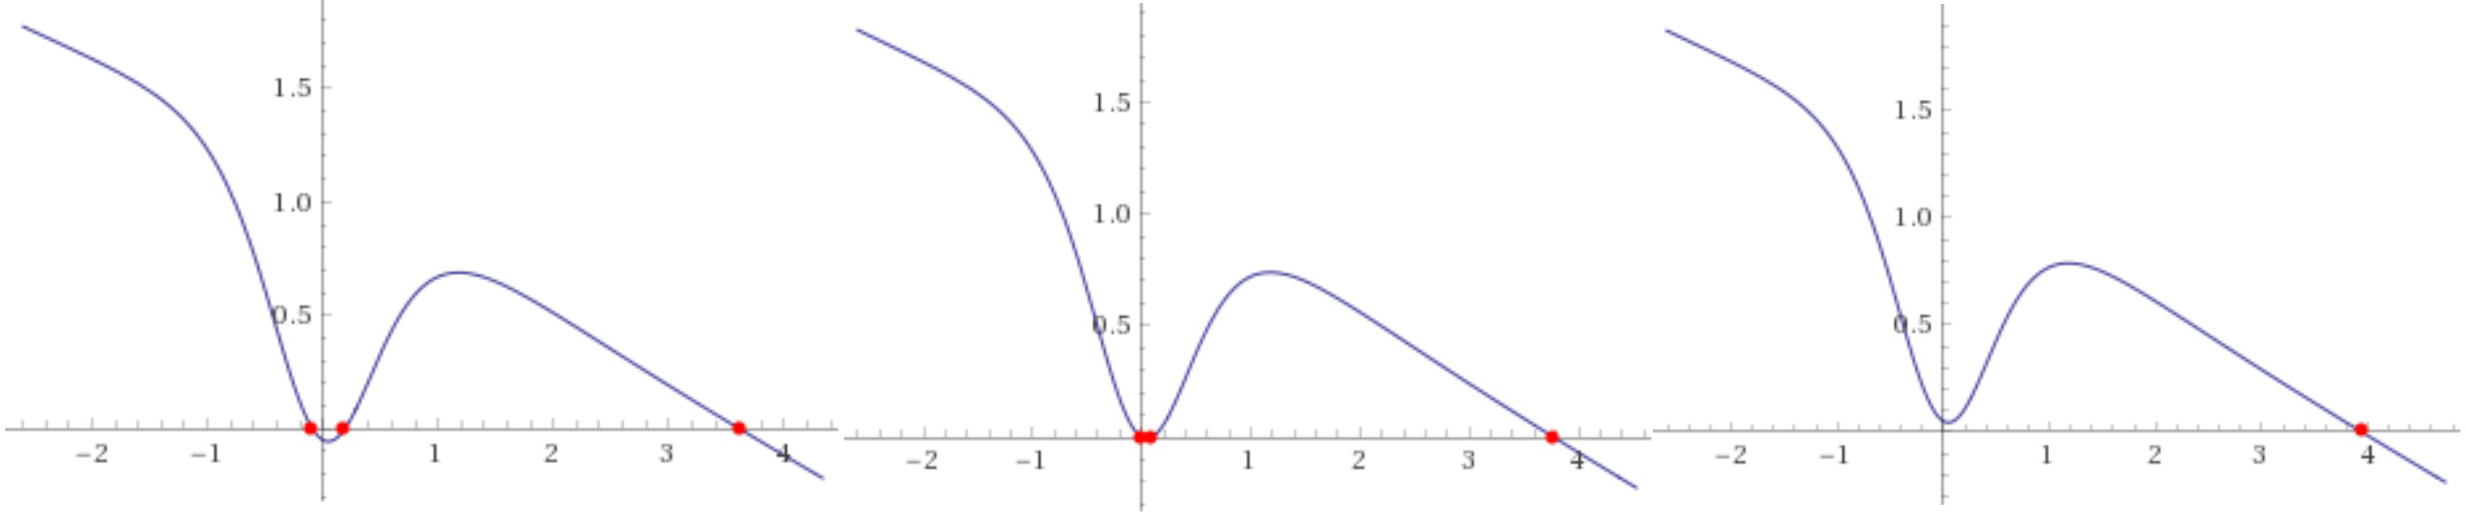
\includegraphics[width=\textwidth]{pic.jpg}
\caption{Left: $\beta=0.95$, middle: $\beta=1$, right: $\beta=1.05$}
\end{figure}


\end{document}
